\scanpage{73}
% archive foliation: 72
$S$ \inserted{lisse} de \deleted{\unsure{t}} type fini sur $\mathbf{F}_p$.

$M$ motif \unsure{ct tordu|et tordu} de poids $\rho$
\margin{? ---}
\[
H^*(S,M_\ell)\overset{\deleted{\unsure{?}}}{\Longleftarrow}H^p(\mathbf{F}_p,R^qf_*(M_\ell))
\]
\diagram{\begin{tikzcd}[column sep=small]
0\arrow[r]&\underbrace{H^{i-1}(\overline{S},\overline{M}_\ell)_\pi}_{\substack{\text{poids entre}\\\rho+i-1\text{ et }\rho+\mathrm{Inf}(\unsure{2i-2|2i},2n)}}\arrow[r]&H^i(S,M_\ell)\arrow[r]&\underbrace{H^i(\overline{S},\overline{M}_\ell)^\pi}_{\substack{\text{poids entre}\\\rho+i\text{ et }\rho+\mathrm{Inf}(2i,2n)}}\arrow[r,dash]&0
\end{tikzcd}}
Donc $H^i(S,M_\ell)=0$ \deleted{\unsure{si on a}} sauf si on a
\[
\rho+i-1\le0\le\rho+2i-2\quad\uline{\text{ou}}\quad\rho+i\le0\le\rho+2i
\]
i.e.
\[
2-2i\le\rho\le\deleted{\unsure{2}}1-i\quad\uline{\text{ou}}\quad-2i\le\rho\le-i
\]
i.e.
\[
\begin{array}{ll}
-2i\le\rho\le-i+1&(\deleted{\unsure{\{}}\text{ si }i\ge2)\\
-2\le\rho\le1&(\text{si }i=1)\\
\rho=0&(\text{si }i=0)
\end{array}
\]
\deleted{Pour $i=1$, on \unsure{trouve}}
\[
\unsure{\rho}
\]
\figure{\begin{tikzpicture}[x=8mm,y=8mm]
\draw (0,0)--(4,0);\draw (0,-.13)--(0,.13);\draw (.6,-.02)--(.6,.3);\draw (3.5,-.12)--(3.5,.3);\draw (4,0)--(4,.15);
\node[below] at (0,-.25) {$-2i$};\node[above] at (.6,.35) {$-2i+2$};\node[below] at (3.5,-.2) {$-i$};\node[above] at (4,.35) {$-i+1$};
\end{tikzpicture}}
\deleted{\figure{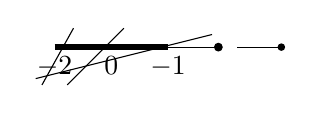
\begin{tikzpicture}[x=8mm,y=8mm]
\draw[line width=2pt] (0,0)--(1.8,0);\draw (1.8,0)--(2.6,0);\draw (2.9,0)--(3.6,0);\fill (2.6,0) circle(.07);\fill (3.6,0) circle(.06);
\node[below] at (0,0) {$-2$};\node[below] at (.9,0) {$\unsure{0}$};\node[below] at (1.8,0) {$-1$};
\draw (-.2,-.6)--(.3,.3);\draw (-.3,-.5)--(2.5,.2);\draw (.2,-.6)--(1.1,.3);
\end{tikzpicture}}}
\figure{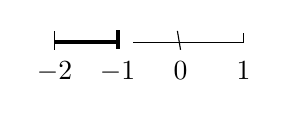
\begin{tikzpicture}[x=8mm,y=8mm]
\draw[line width=1.4pt] (0,0)--(1,0);\draw (1.25,0)--(3,0);\draw (0,-.12)--(0,.18);\draw[line width=1.4pt] (1,-.1)--(1,.2);\draw (2,-.12)--(1.95,.18);\draw (3,0)--(3,.15);
\node[below] at (0,-.15) {$-2$};\node[below] at (1,-.15) {$-1$};\node[below] at (2,-.15) {$0$};\node[below] at (3,-.15) {$1$};
\end{tikzpicture}}
